% !TEX root=frame_thesis.tex
\chapter{Results}

\section{Standard Run}
The standard run of the ABM presented in Section \ref{chapter:Methods} aims to proof the general functioning and coherence of the model.
The simulation with parameter settings given in Table \ref{tab:sensitivity} is performed with five different seeds and the resulting ensemble mean and standard deviation of aggregated variables are shown in Figure \ref{fig:STDstats}.
The spatial patterns of tree cover, farming and settlements at different times of one single run are shown in Figure \ref{fig:STDrull}.
The uncertainty of the ensemble run results from slight differences in the timing of the dynamics due to different realisations of the discrete, stochastic population growth process (see also Figure \ref{fig:realisationsofpopgrowth}).

\begin{figure}
	\centering
	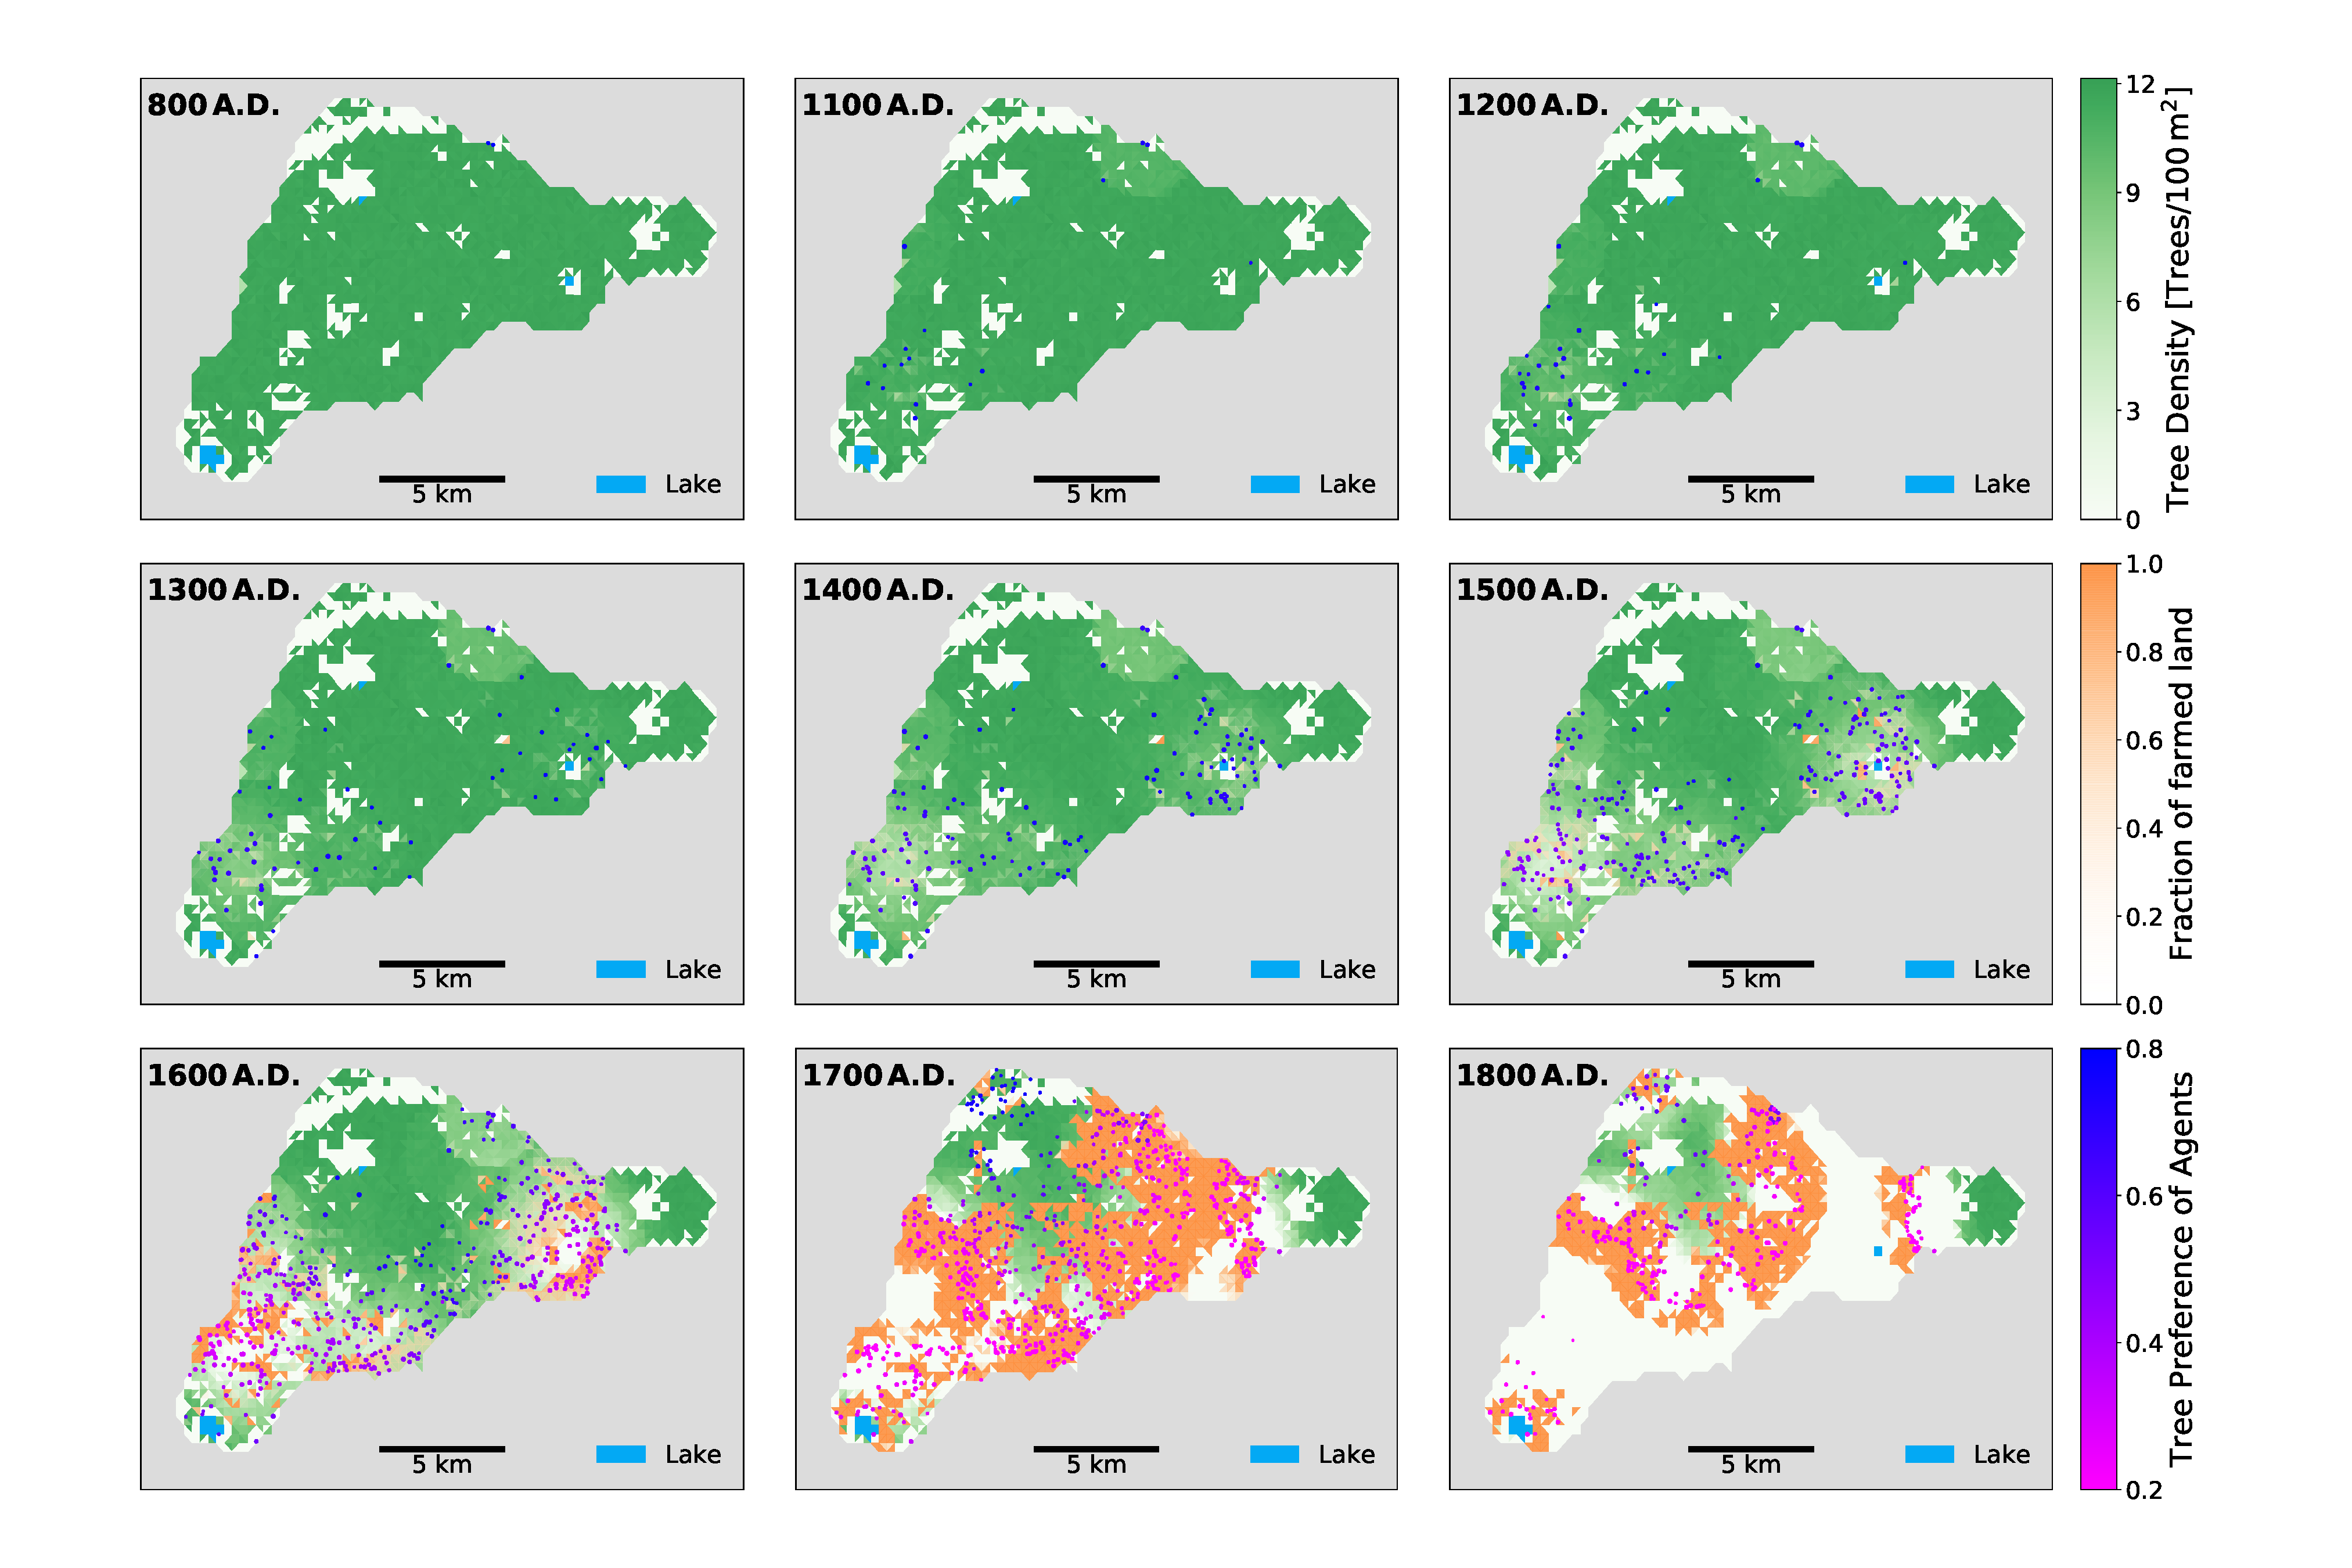
\includegraphics[width=1.5\textwidth, center]{images/Results/Standard/Rull2020_Comparison_seed3}
	\caption{The spatial patterns of for snapshots at 9 different times.}
	\label{fig:STDrull}
\end{figure}


\begin{figure}
	\centering
	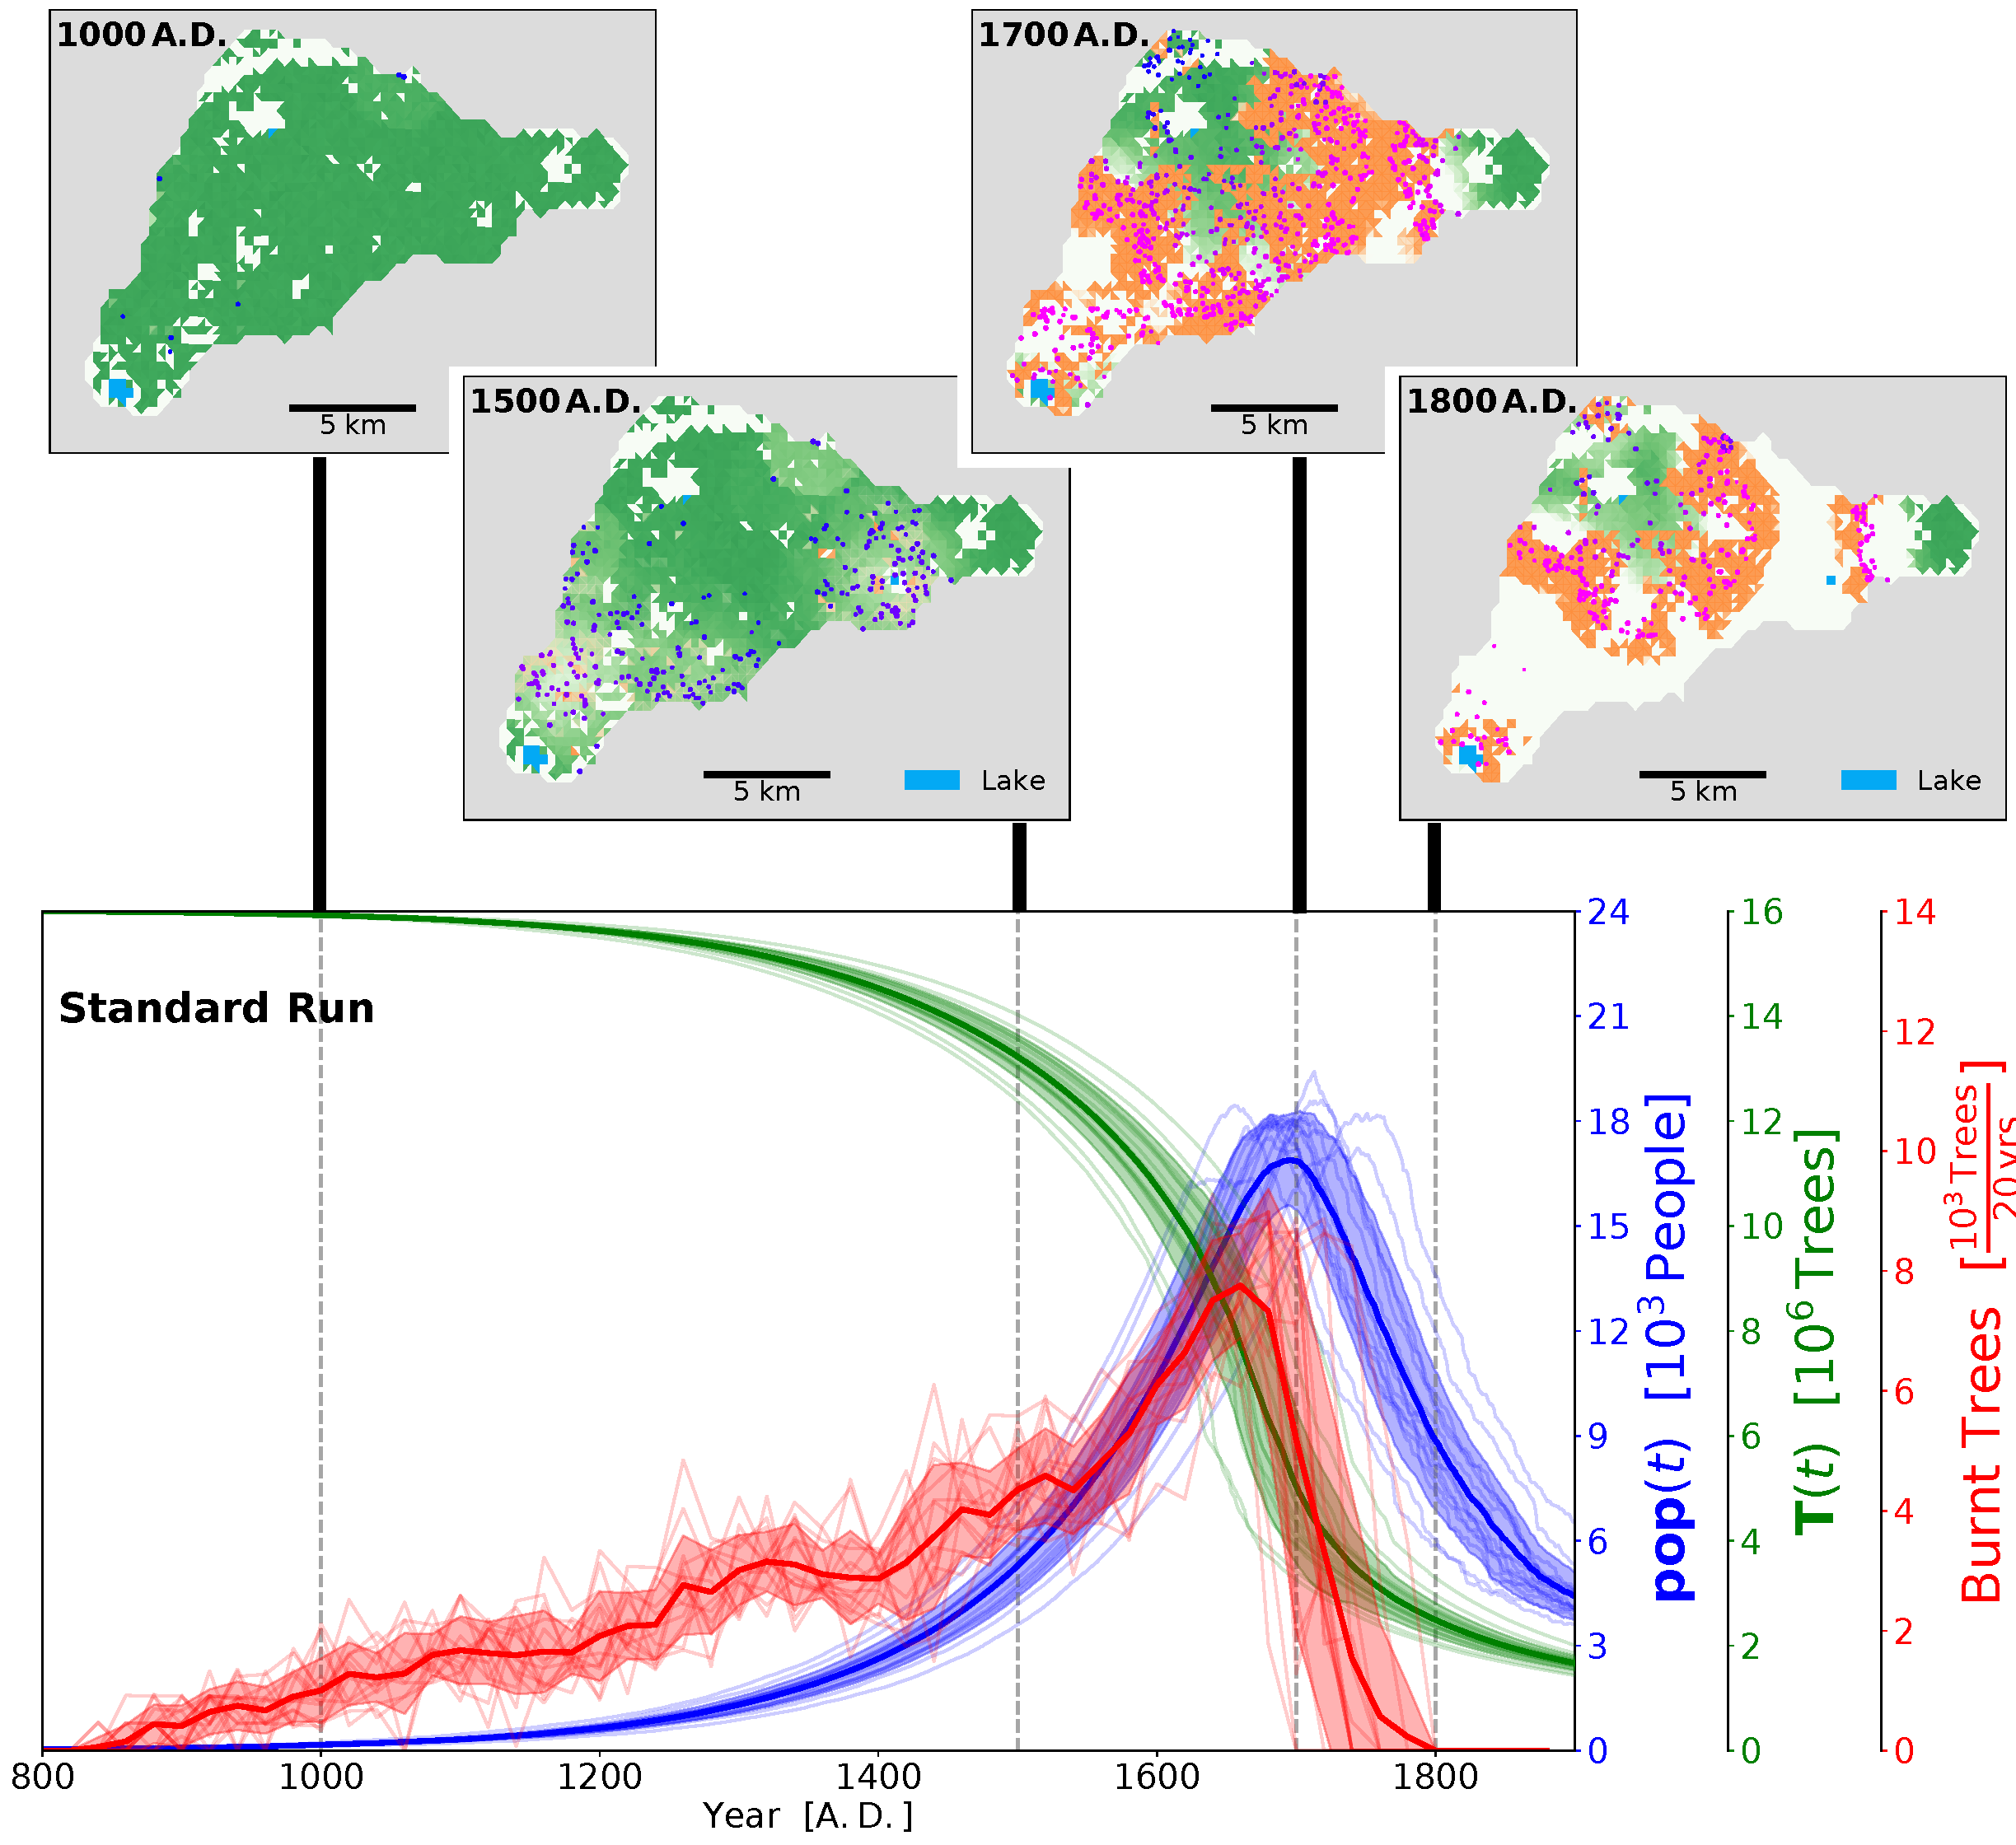
\includegraphics[width=1.3\linewidth, center]{images/Results/Standard/EnsembleStatistics+Panels}
	\caption{Dynamics of aggregate population size, trees, and burnt trees with standard setting of parameters. Five different realisations are used to obtain the ensemble mean and standard deviation (shaded area). The panels above show the spatial distribution of trees, farming and agent settlements with their tree preferences for one of these realisations (with the same scale as in Figure \ref{fig:STDrull}). }
	\label{fig:STDstats}
\end{figure}


The results replicate in general the expected behaviour, which is described in the remaining section. 
In the beginning of the simulation agents settle at Anakena Beach (in the North). 
The local tree density is at the carrying capacity and thus the agents' tree preference high (blue colour).
The agents' population size grows at a constant maximum growth rate, because trees and arable land are both abundant. 
Consequently, groups of individuals split, form new agents and start to settle the rest of the island.
Until the end of the first drought period in $1200\, {\rm A.D.}$, new agents tend to settle in the arable, coastal region South/South East of the island in close proximity to the major freshwater source Rano Kau with low penalties for geography, freshwater distance. 
With population density on the rise, deforestation and farming activity in this region intensify.
After $1200\, {\rm A.D.}$, also the region around Rano Raraku, now providing an alternative freshwater source, is settled at quick pace.
%At $1200\,{\rm A.D.}$, the drought period ends and Rano Raraku (in the West) provides another freshwater source, causing many new agents to move to the South West and North West coast.
%With ever increasing population density, especially in these centres, 
Agents adapt to the slow environmental change with a linearly decreasing tree preference and, thus, intensified farming activity.
As Figure \ref{fig:STDstats} shows, the amount of burnt trees to clear land for agriculture in a 20 year time window also increases linearly until $1550\, {\rm A.D}$.
%, followed by a sharp increase around 1650.
%At peak, roughly $10\cdot 10^3$ trees are cleared in a 20 year period in order to fill the agents' farming requirement.

\begin{figure}
	\centering
	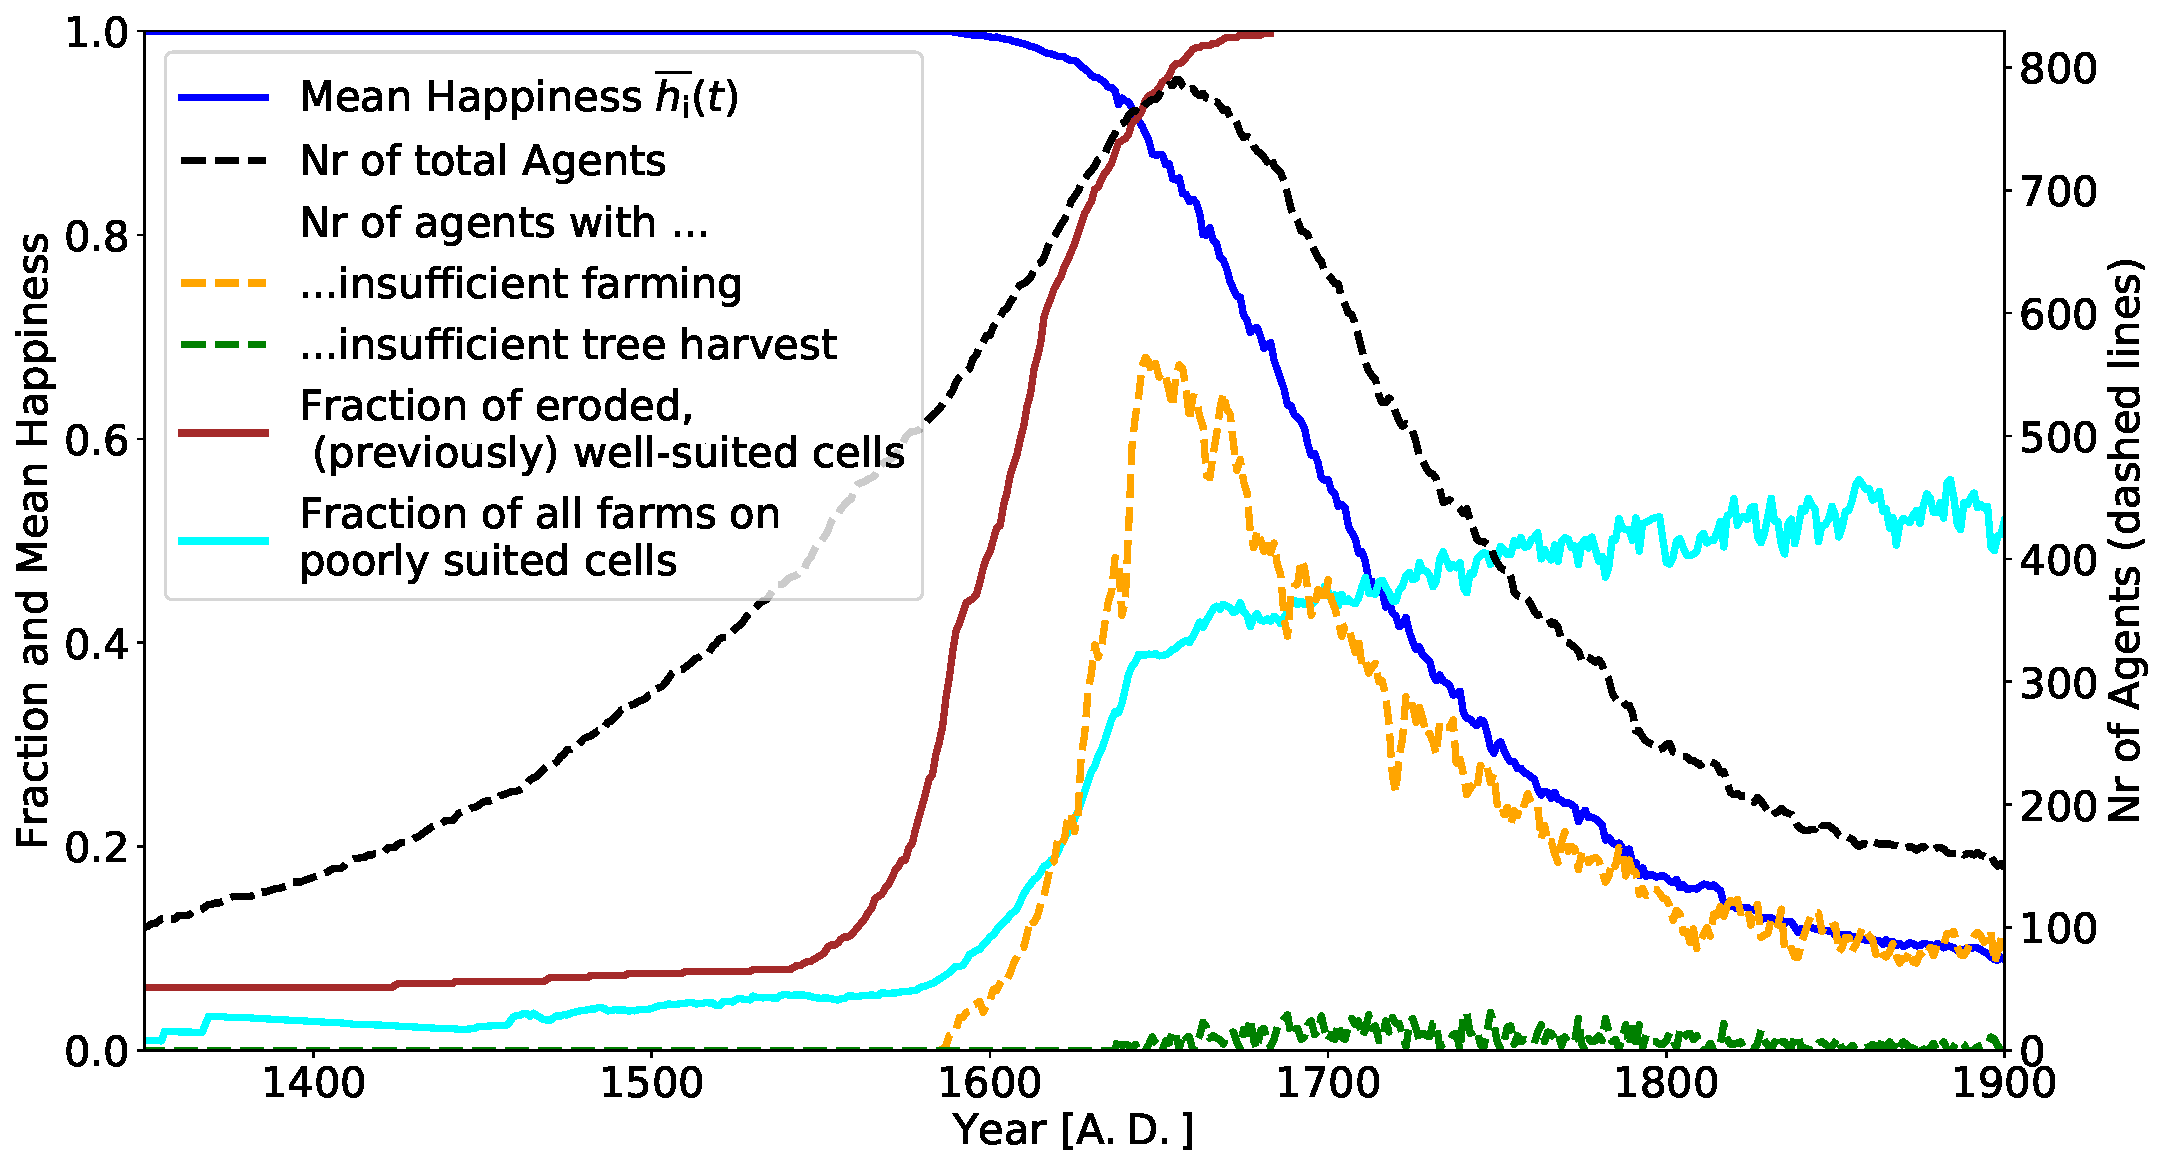
\includegraphics[width=\textwidth]{images/Results/Standard/STDsecondaryStats}
	\caption{The plot shows the development and causes of the change from net growth to net decline in Easter Island population dynamics for one single realisation in the Standard setting.
	Dashed lines correspond to the axis on the right giving absolute number of agents.
	The blue line shows the mean happiness index of all living agents. The black, dashed line shows the total number of agents. The number of agents that lack either sufficient available land for farming or trees are shown in yellow and green. The brown line shows the fraction of cells that previously classified as well-suited for farming but after complete deforestation eroded is shown. The cyan line shows the fraction of farming sites (of all agents) on poorly suited sites.
	The development is described in detail in the main text.}
	\label{fig:STDsecondayrstats}
\end{figure}

%Thereby, agents accelerate the depletion of the non-renewable resource, trees and, thus, in a self-enhancing loop, acquire more farming land.

%Further, this large-scale deforestation leads to a sharp increase of erosion of well-suited sites around $1650\, {\rm A.D.}$ and, hence, agents can not fill their farming requirements.

% with the first agents not meeting their resource requirements.
%However, since both neither further arable sites are available in the densely populated coastal regions and trees are deforested entirely by the remaining agents, these previously well-suited settlement locations are abandoned and the agents turn to the mostly poorly suited upland areas causing a shift towards the interior of the island.
%With the first agents not meeting their farming requirements around 1650, occupation of upland poorly suited farming sites jumps from a negligible fraction in $1650$ to $40-59\%$ in 1700.
%Consequently, the amount of burned trees rises quickly and comes to a abrupt halt between 1700 and 1800.
%Due to the low productivity indices of these sites, the use of burning trees to clear more space rises sharply in this period.


In a self-enhancing loop, population growth in the settlement centres leads to an intensification of deforestation, a consequent decrease of the agents' tree preferences, increase of farming requirements, more acquisition of farming sites (therefore, more burnt trees) and, ultimately, again increased intensification of deforestation.
Simultaneously, erosion further accelerates the deforestation as farming productivity indices decrease and more farming sites per agent need to be acquired.
%of arable farming land increases, leading to declined farming efficiency and, thus, more farming sites required per agent.
The number of eroded, (previously) well-suited cells jumps from less than $10\%$ of all well-suited sites in $1600\,{\rm A.D.}$ to $100\%$ by $1700\, {\rm A.D.}$ (brown curve in Figure \ref{fig:STDsecondayrstats}).
Consequently, in this period the amount of trees burnt for clearing new land rises sharply to roughly $8\cdot 10^3$ trees per $20 \, {\rm yrs}$.
In total, this acceleration of the local resource scarcity, leads to an abandonment of the previously well-suited settlement locations starting in $1650\,{\rm A.D.}$ and the agents turn to the mostly poorly suited, interior, upland areas.
The share of farming activity on those poorly suited cells rises from a negligible fraction in $1650\, {\rm A.D.}$ to $40\%$ of all farming activity in $1700\,{\rm A.D.}$ (cyan line in Figure \ref{fig:STDsecondayrstats}).
%However, the lower productivity indices in the poorly suited sites, leads to a further increase in land acquisition and, thus, deforestation. 

While in $1700\,{\rm A.D.}$ more than half of the agents experience some minor shortage in farming produce, the loss of the non-renewable resource trees for some agents is what sets in an exponential decline of the mean happiness, $\overline{h_{\rm i}(t)}$ just after $1700\, {\rm A.D.}$ (blue line in Figure \ref{fig:STDsecondayrstats}).
This also marks the end of the net exponential growth of the population size, which peaks at around $18\cdot 10^3$ people.
Within a relative short time period of less than $50$ years, the population starts to decrease exponentially with a rate of around $-0.5$ to $-1\%$ (see Figure \ref{fig:app:STDnetgrowthrate}).
There is neither insufficient farming land, nor insufficient trees on the island.
It is rather that all locations on the map lacks one or the other resource in its local surrounding.
For agents that want to move, no valid locations are available that fulfil both resource requirements, consequently, their memory happiness, $H_{\rm i}(t)$ quickly drops to $0$ and the agent vanishes.
As the population size decreases significantly and consequently burning of trees stops, the deforestation level slows down around $1750\, {\rm A.D.}$ at slightly less than $25\%$ of the initial total number of trees. 
%have not enough farming sites with a happiness $H_{\rm i}(t)>H_{\rm equ}$ and therefore positive net growth. 
%The agents unable to find enough trees to cut, however, at this point of time quickly vanish as there are no valid locations to settle anymore and no replacement leading to a memory happiness of $H_{\rm i}(t) = 0$ very quickly.
%Finally, by $1800\,{\rm A.D.}$, the population decrease slows down. 
%The net population growth is shown in Figure \ref{fig:app:STDnetgrowthrate}. 
There is no stable coexistence of population and trees number in this scenario setting as tree regeneration rate is disabled and, hence, the agents rely on an entirely non-renewable resource.
Population size declines further until no agents are left.



%especially cultivation of poorly suited sites, which in turn increases the fires and amplifying the development.
%In turn, sharp increase of fires around $1600\, {\rm A.D.}$. 
%Around $1650\, {\rm A.D.}$, constant exponential growth stops, population size remains constant for a short period and, finally, decays exponentially.
%This coincides with a steep increase of agents with not enough available farming productivity causing the mean happiness to decline. 
%As shown in Figure \ref{fig:happyStd}
%However, only when trees become scarce in the region



% \begin{itemize}
% 	\item Fig 2: Aggregate Dynamics (population, trees, mean penalties and happiness, fires, excess mortality/fertility). The plot that Esteban sketched during last Zoom Meeting [called statistics plot from now on]. All statistics plots are mean ensemble runs of 5 different seeds.
% 	\item Fig 1: Comparison of the spatial deforestation pattern with \citet{Rull2020}'s Figure, which we sent to Valenti.
% \end{itemize}


%The dynamics of population size $\mathbf{pop}(t)$, total number of trees $\mathbf{T}(t)$ and amount of burnt trees in a 20 year time period) are shown in Figure \ref{fig:STDstats}. 
%For the first $850\, {\rm yrs}$ after arrival, the population grows exponentially.
%Then, around $1650\, {\rm A.D.}$ the dynamics change significantly, leading to a significant population size reduction after $1750\, {\rm A.D.}$.
%The rate of population size decrease is ....\TODO (i.e.\ the number of $g(H_{\rm i}(t))$ for agents $i$ and $t>1750\, {\rm A.D.}$ is on average ... \TODO.).


%
%We can look 
%Figure \ref{fig:app:treefillfarmfillmoves} 

\section{Different theories}
%Statistics Plots for a
%\begin{itemize}
%	\item Run with low N fixation (instead of high)
%	\item Run with tree regeneration and high N fixation
%	\item Run with tree regeneration and low N fixation
%\end{itemize}
%In the making

The standard setting used for this model reproduces a boom and bust cycle, with a population decline rate in the order of the initial growth rate.
By allowing for tree regeneration and/or changing the amount of required farmed land for one person, $F_\text{Req, pP}$, I obtain very contrary results leading to alternative interpretations of the population dynamics in the model.
Figure \ref{fig:TheoriesStats} shows four different scenarios:
\begin{itemize}
	\item The upper left panel is again the Standard Run (using the high Nitrogen fixation scenario in \citet{Puleston2017} for $F_\text{Req, pP}$ and disabled tree regeneration) shown in Figure \ref{fig:STDstats} for comparison.
	\item In the upper right panel, I choose the low Nitrogen fixation by  \citet{Puleston2017} with much higher requirement of farmed land per person.
	Population peaks at a smaller number ($\TODO$) and the decrease in population is slower with a rates \TODO.
	The amount of burnt trees especially in the first phase with constant population growth rate is much higher in this scenario, because more arable land needs to be occupied by the agents for similar amount of populations.
	\item In the bottom panels, tree regeneration is enabled with parameters set as in Table \ref{tab:sensitivity}. The bottom left panel corresponds to the high, the bottom right to the low Nitrogen fixation scenario.
	Population rises similarly in the first phase of the dynamics as in the case without tree regeneration. However, a population maximum occurs later and at respectively higher levels. When the maximum carrying capacity is reached, population decreases slowly and levels off at an equilibrium value for both scenarios, in which the renewal of trees matches the requirement of the population and the amount of farming land required remains constant.
\end{itemize}
All panels show mean values obtained from an ensemble of five runs.

In the supplementary material, I provide movies showing the spatial settlement behaviour of single realisations of the different scenarios described above.

If tree regrowth is enabled over time all arable cells are turned into farming sites and trees are obtained from non-viable sites.
An heterogeneous pattern of agents with different tree preferences emerges with some areas dominated by agents at maximum, some at minimum tree preference.
 pattern of areas with high tree densities and high farming densities is obtained. 
\TODO!!

\begin{figure}
	\centering
	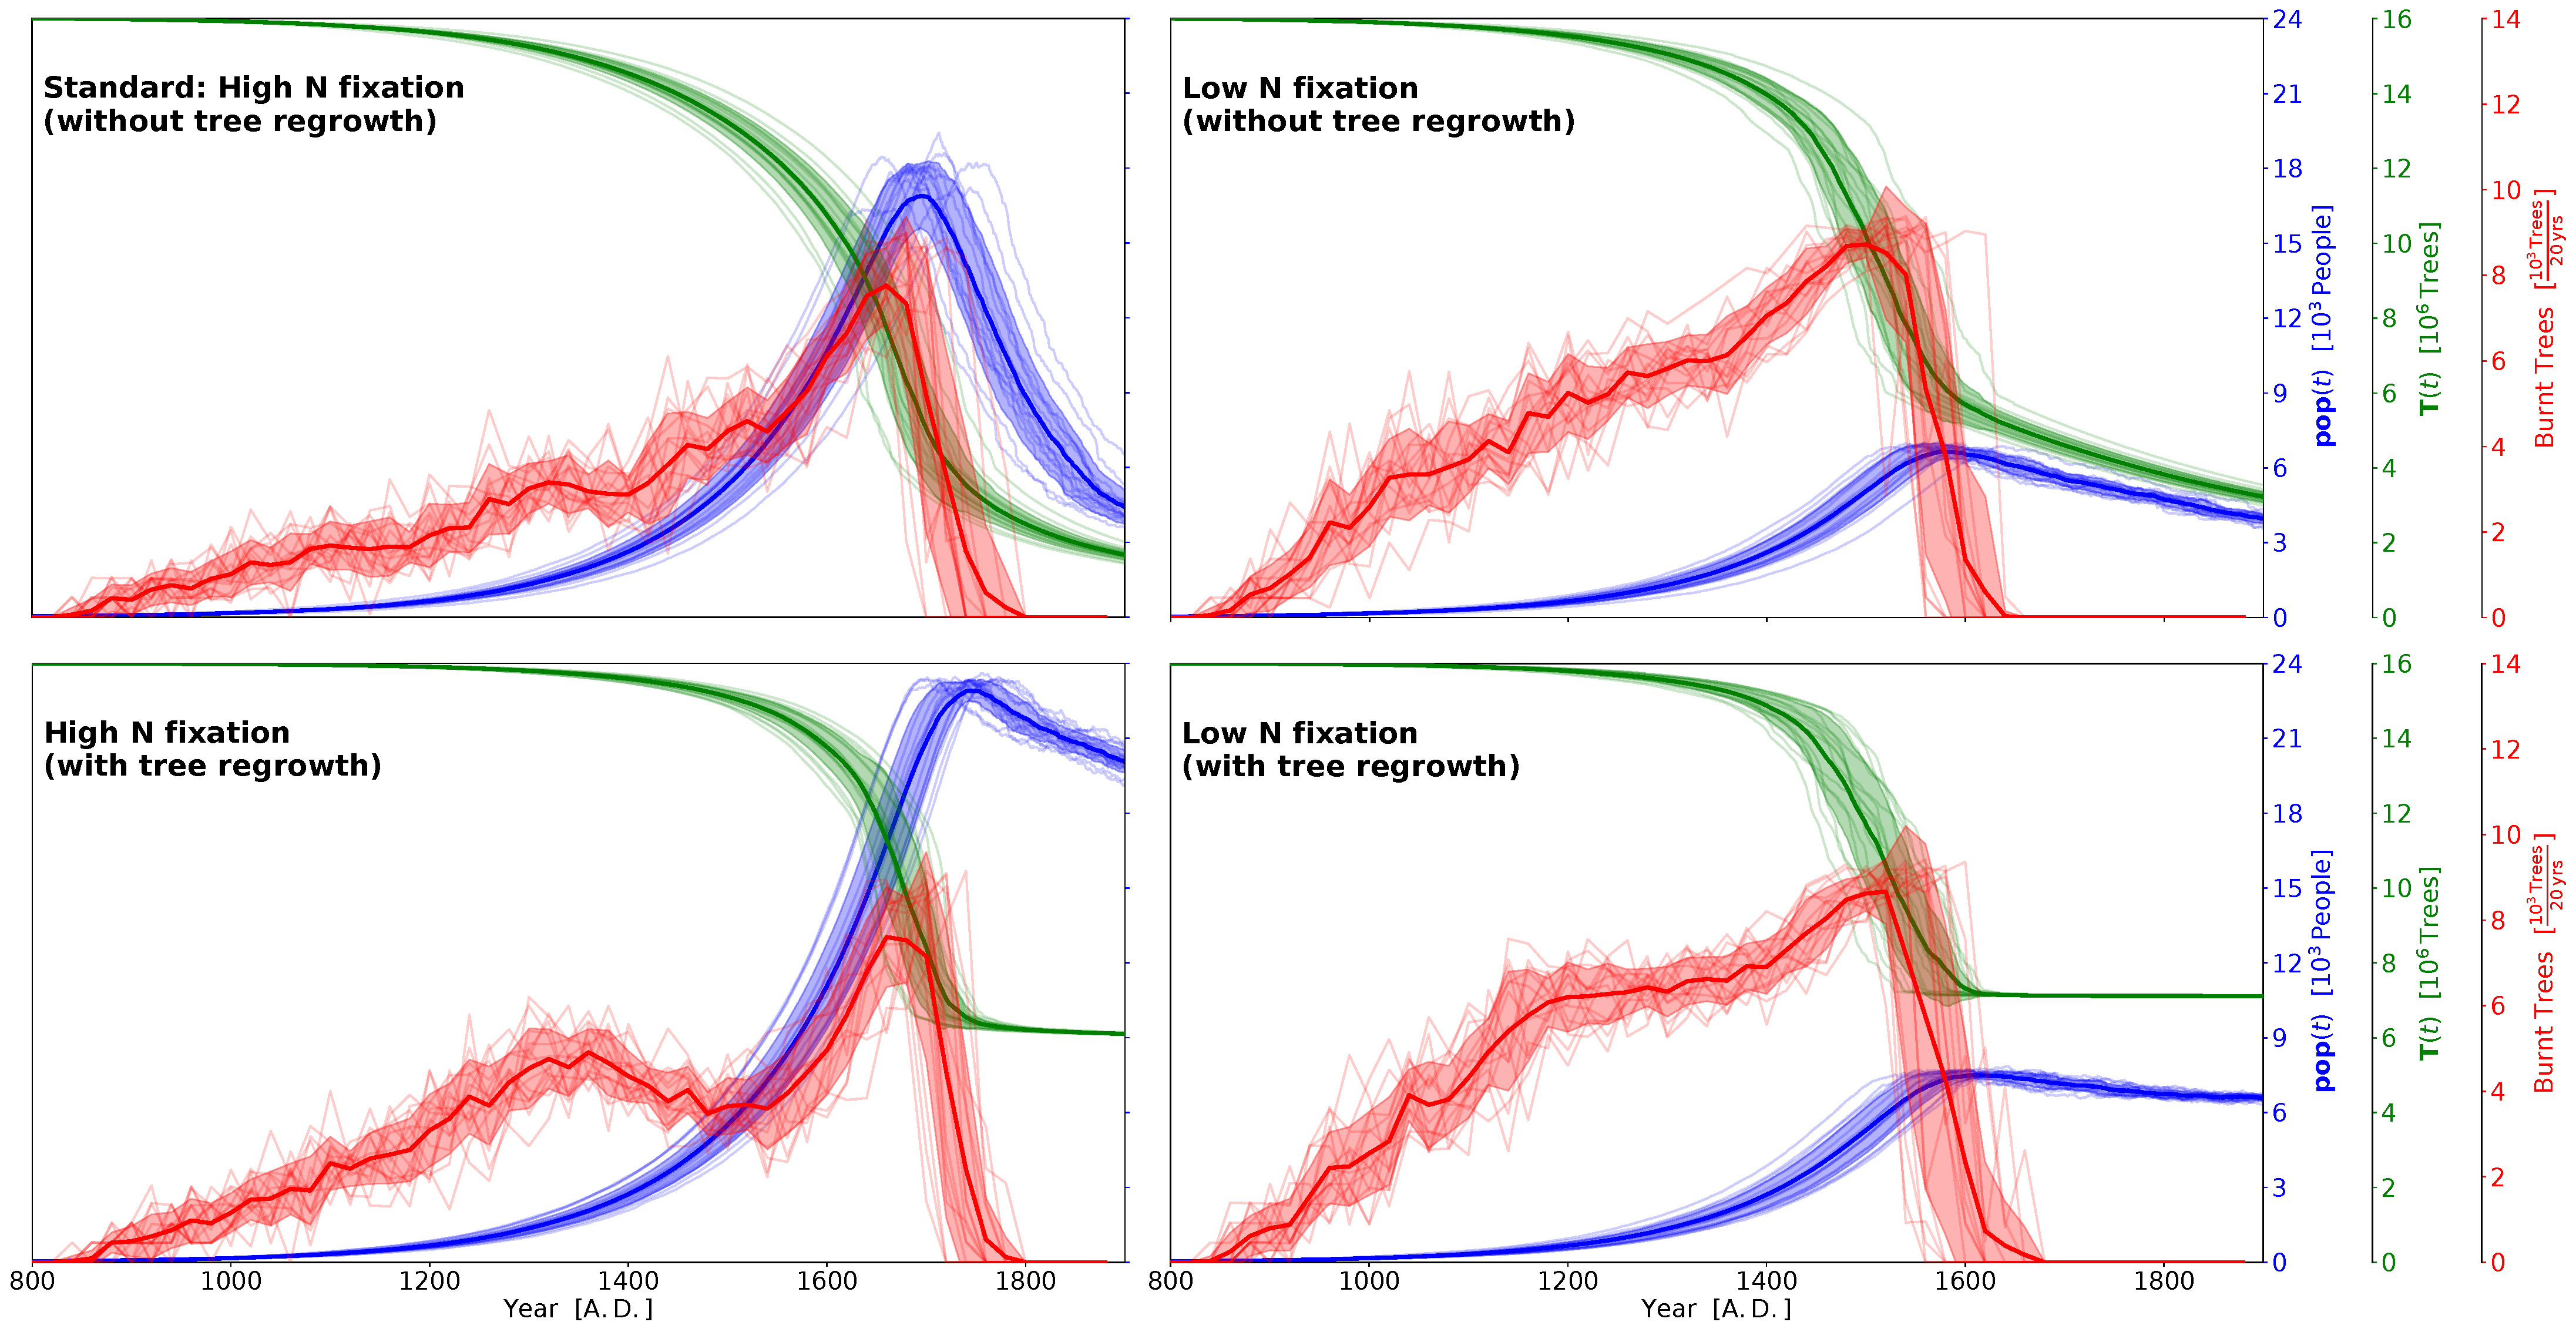
\includegraphics[width=1.3\textwidth, center]{images/Results/Standard/EnsembleStatistics_allTheories}
	\caption{}
	\label{fig:ensemblestatisticsalltheories}
\end{figure}



\section{Different Tree Preference Functions, i.e.\ Agent Adaption}
\begin{itemize}
	\item Runs with $f_{\rm Tree \ Pref}$ delayed, careful, logistic.
\end{itemize}
I don't know yet if this makes any difference to the standard run and what difference. So we'll see.

Tree, Burn, Pop TPREF!!!


\section{A less resilient society}
Run with a larger shape parameter of $g(H_{\rm i})(t)$.
I don't know yet if this makes any difference to the standard run and what difference. So we'll see.
I assume that the turning point of growing population to decreasing population size happens earlier. Maybe I'll just show the statistics plot.


\section{Senstivity Analysis of some uncertain parameters}
$r_{\rm T}$, $r_{\rm F}$,
$T_{\rm Req, pP}$

\section{Three different decision making processes}
\begin{itemize}
	\item Standard setting, $\gamma=20$, $\alpha=(0.2,0.2,0.2,0.2,0.2)$.
	\item `Only resource availability matters for moving decision' setting, $\gamma=20$, $\alpha=(0, 0, 0, 0.5,0.5)$.
	\item Hopping agents, that move to a random spot with uniform probability over the island, $\gamma=0$, $\alpha=$ doesn't matter.
\end{itemize}
Results not yet known. I guess I'll describe qualitatively what happens to the spatial patterns. 
If the aggregate dynamics change, this would of course be a big, big result and I would focus on that.


\section{Regional Dynamics}
There is strong regional variation in the dynamics of Easter Island population dynamics as well as deforestation pattern. 
Figure \ref{fig:mapregionscoarse} shows a division of the island into seven different regions, with common geographical features (in anti-clockwise order): The area around the crater lake Rano Kau, the south coast, the area around Rano Raraku, the area around Anakena Beach, the steep North West Coast, the fertile area where today's main town, Hanga Roa, is located, and the upland area including Poike Peninsula. 
I allocate the cells to each of these regions by choosing centres of these regions or several sub regions by hand and then defining a region by the corresponding Voroni cell.

\begin{figure}
	\centering
	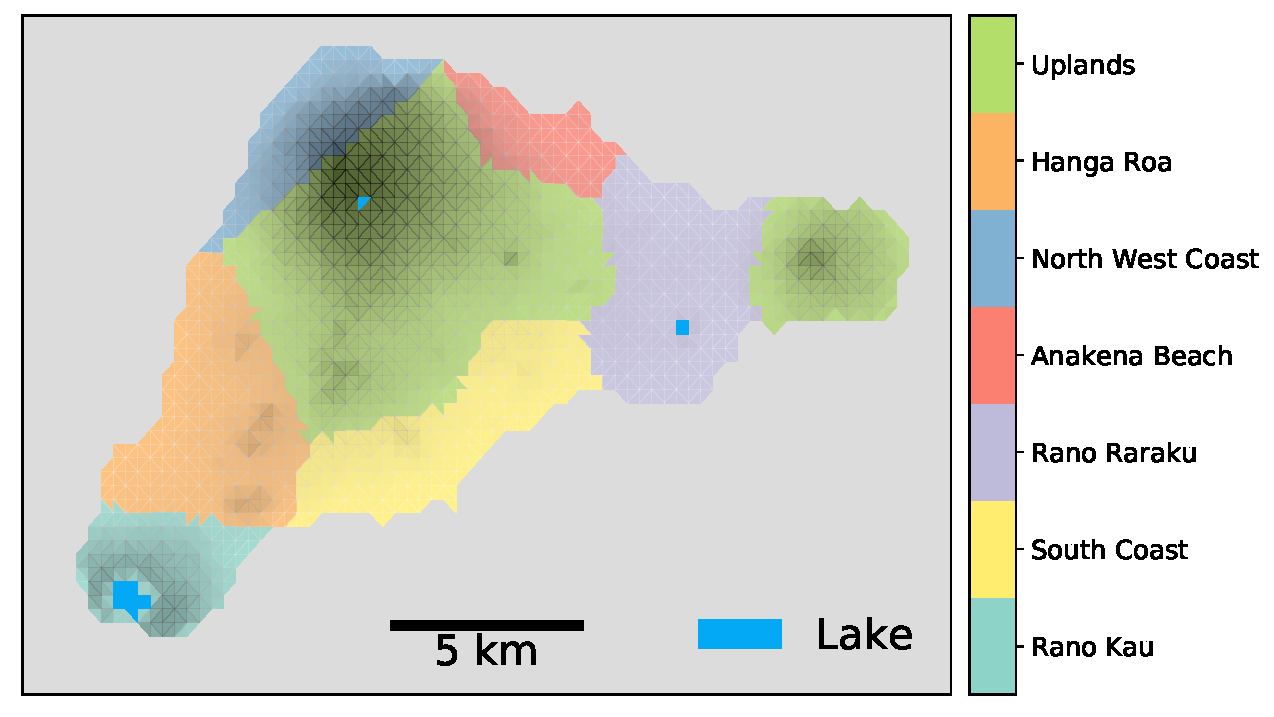
\includegraphics[width=1.0\linewidth]{images/Results/Standard/MapRegionsCoarse}
	\caption{Division of the map into seven separate regions.}
	\label{fig:mapregionscoarse}
\end{figure}

The population dynamics of each region varies strongly. 
Some regions like Hanga Roa and Rano Raraku (with a little delay) show early extensive growth followed by a steep decline of population.
In others, the population declines less dramatically after reaching a peak, e.g.\ in the South Coast or the Uplands 

The small, less arable regions at Rano Kau, the North West Coast, or Anakena Beach, show some population growth after other, more favourable regions are abandoned and then decline slow and linearly or in the case of Rano Kau remain at the same population size for nearly $200$ years.

\begin{figure}
	\centering
	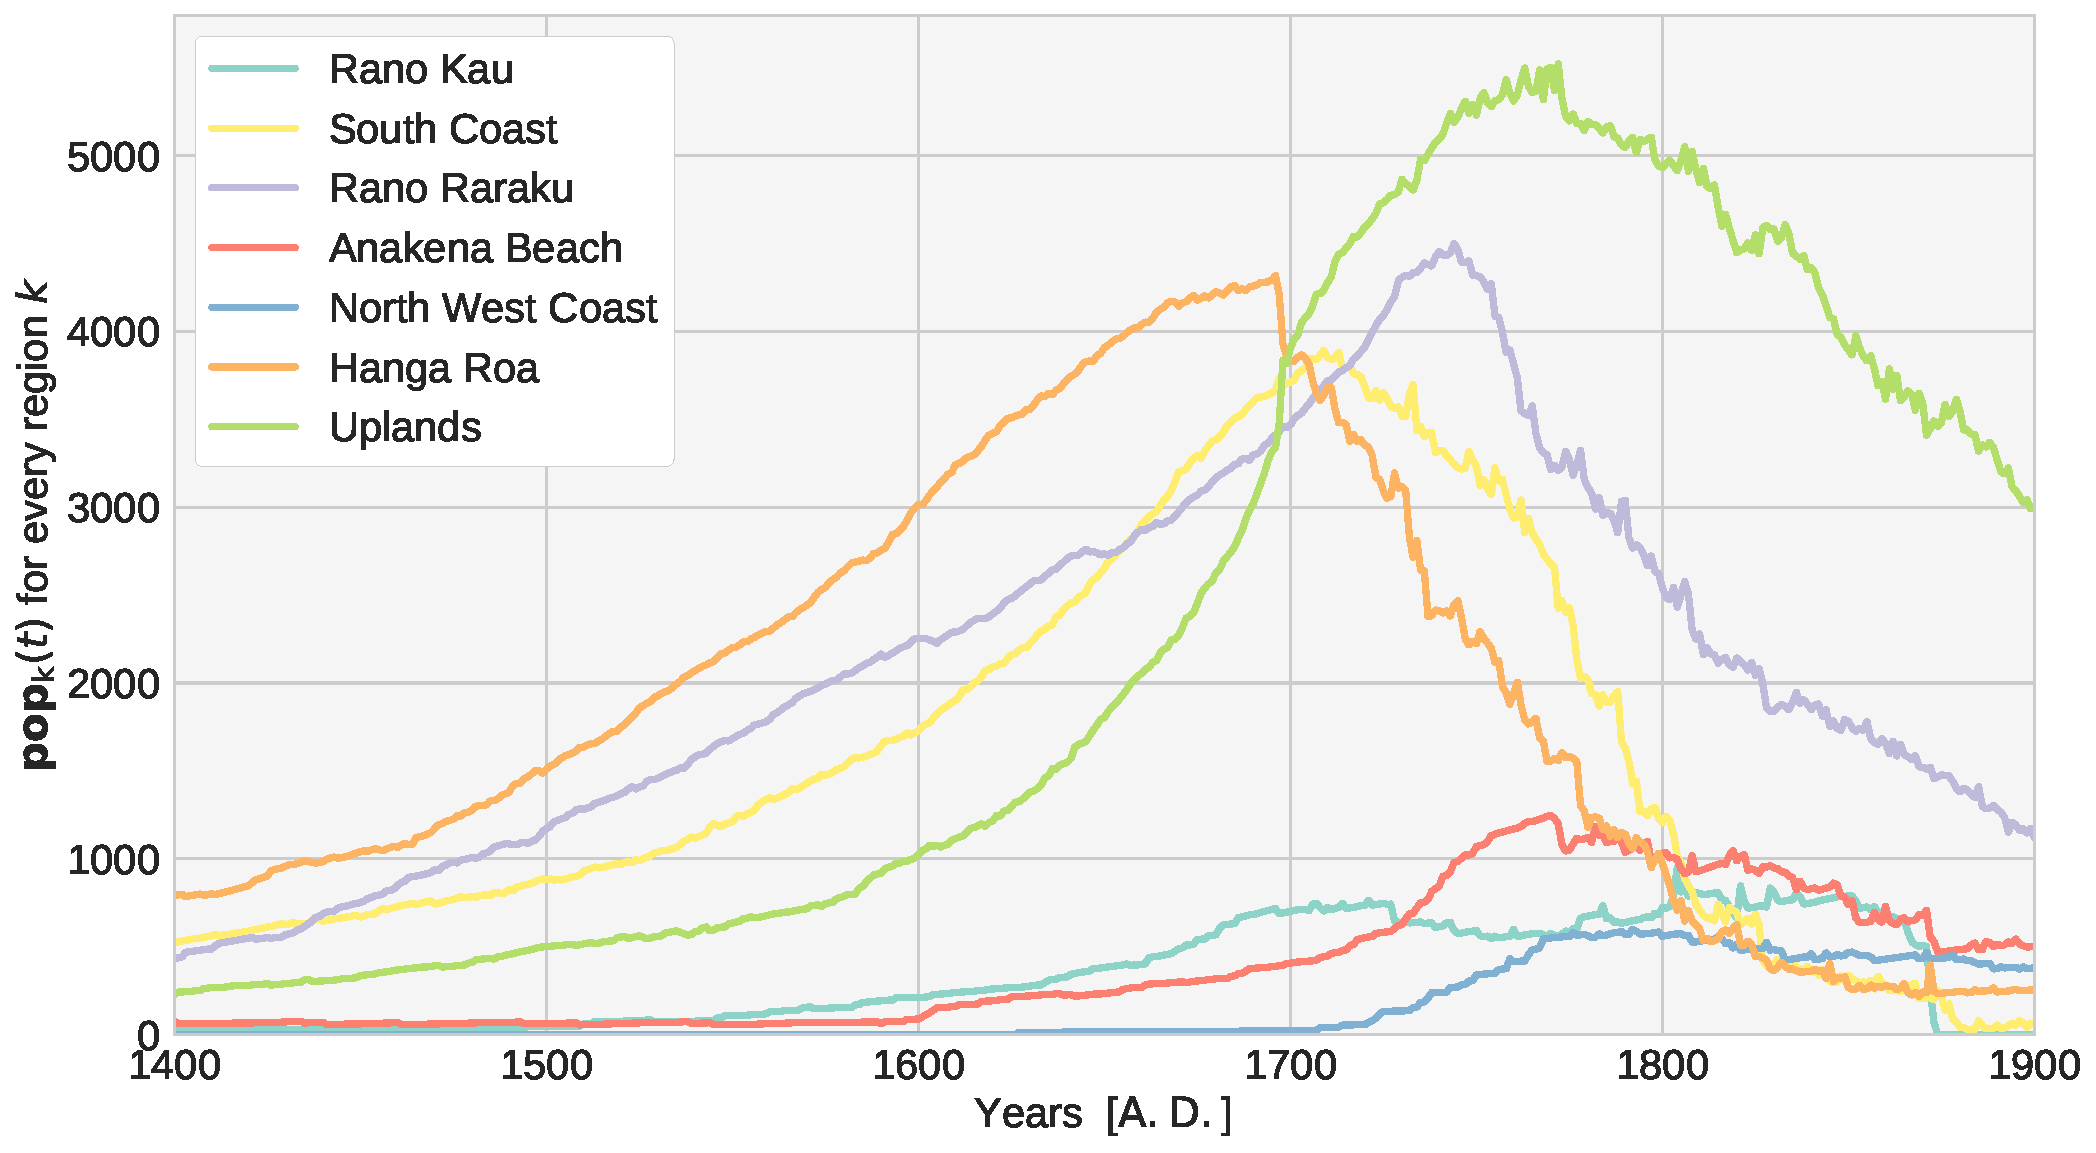
\includegraphics[width=1.0\linewidth]{images/Results/Standard/RegionalStats}
	\caption{The population dynamics of each separate region defined in Figure \ref{fig:mapregionscoarse}.}
	\label{fig:regionalstats}
\end{figure}

\section{Fires}
Plot the distribution of fires on the map over time. 
I imagine a map in which the color determines the timing of fires in each cell. 
I'm not sure yet how to do this exactly since fires in any cell occur at multiple times. Maybe I'll take the first occurence. We'll see.



\chapter{Discussion and Conclusion}
